\documentclass[conference]{IEEEtran}
\usepackage{cite}
\usepackage{amsmath,amssymb,amsfonts}
\usepackage{graphicx}
\usepackage{booktabs}
\usepackage{algorithm}
\usepackage{algpseudocode}
\usepackage{textcomp}
\usepackage{xcolor}
\usepackage[hidelinks]{hyperref}

\begin{document}

% Replace with your title. Keep formulas and unexplained abbreviations out of it.
\title{Low-Power Occupancy Sensing for Smart Buildings Using Edge-Deployed Neural Networks}

% One block per author: copy a block to add an author, delete one to remove an author.
\author{\IEEEauthorblockN{Priya Raman}
\IEEEauthorblockA{\textit{Dept. of Electrical Engineering} \\
\textit{Northfield Institute of Technology}\\
Pune, India \\
priya.raman@northfield.example}
\and
\IEEEauthorblockN{Daniel Okafor}
\IEEEauthorblockA{\textit{Dept. of Computer Science} \\
\textit{Northfield Institute of Technology}\\
Pune, India \\
daniel.okafor@northfield.example}
\and
\IEEEauthorblockN{Mei Tanaka}
\IEEEauthorblockA{\textit{Building Systems Group} \\
\textit{Harbour Automation Ltd.}\\
Osaka, Japan \\
m.tanaka@harbour-automation.example}
}

\maketitle

% Replace with your abstract. IEEEtran prints the word "Abstract" for you.
\begin{abstract}
Heating, ventilation and lighting are usually run on fixed schedules, although most rooms in an office are empty for a large part of the day. We present a battery-powered sensor node that estimates how many people are in a room from passive infrared, carbon dioxide and sound-level readings, using a small neural network that runs on the node itself. The network has 4.1 thousand parameters, is quantized to 8-bit integers and needs 38 ms per inference on a microcontroller. In a twelve-week deployment across 14 meeting rooms, the node detected occupancy with 94.2\% accuracy and estimated the number of occupants to within one person in 87.6\% of intervals, while drawing an average of 0.31 mW. Running the ventilation from these estimates reduced fan energy by 23\% compared with the existing schedule.
\end{abstract}

% Replace with three to five keywords.
\begin{IEEEkeywords}
occupancy sensing, embedded machine learning, smart buildings, energy efficiency, sensor fusion
\end{IEEEkeywords}

\section{Introduction}\label{sec:introduction}
Buildings account for roughly a third of final energy use, and a large share of that goes to conditioning and lighting rooms that nobody is in. Office meeting rooms are a clear example: they are booked in blocks, used for part of each booking, and ventilated at a constant rate from early morning until evening. Knowing whether a room is occupied, and by how many people, lets a building controller match fresh-air supply to demand.

Cameras can count people accurately, but they raise privacy concerns and need mains power and network cabling. Simple motion detectors are cheap and private, yet they miss people who sit still and cannot say how many are present. Carbon dioxide concentration follows occupancy, but only after several minutes. No single low-cost sensor is sufficient; combining them is the natural step, and the open question is where the combination should be computed.

This paper argues that it should be computed on the sensor node. Sending raw readings to a server costs radio energy, which dominates the power budget of a battery-powered node, and exposes sound-level traces that occupants may not want to leave the room. Recent work on compact convolutional networks~\cite{howard2017mobilenets} shows that useful models fit in a few kilobytes once they are designed for the task.

Our contributions are as follows.
\begin{itemize}
  \item A sensor node that fuses three inexpensive sensors and runs an 8-bit neural network on a microcontroller, transmitting one small estimate per minute (Section~\ref{sec:methodology}).
  \item A training procedure that keeps accuracy within one percentage point of the floating-point model after quantization.
  \item A twelve-week field study in 14 meeting rooms, with accuracy, power and energy-saving results (Section~\ref{sec:experiments}).
\end{itemize}

\section{Related Work}\label{sec:related-work}
\subsection{Occupancy Sensing}
Early systems used a single passive infrared (PIR) detector with a timeout, which keeps the lights on for a fixed period after the last movement. Later work added carbon dioxide and door sensors and treated occupancy as a classification problem over hand-built features. These approaches run on a central server and assume a wired sensor network.

\subsection{Compact Neural Networks}
Convolutional networks have been the standard tool for learning from sensor and image data since LeNet~\cite{lecun1998gradient}, and residual connections made much deeper models trainable~\cite{he2016deep}. For devices with little memory, depthwise-separable convolutions reduce the parameter count by an order of magnitude at a small cost in accuracy~\cite{howard2017mobilenets}. Recurrent models such as the long short-term memory network~\cite{hochreiter1997long} capture longer histories, but their state does not quantize as cleanly, which is why we use a convolutional model over a fixed window.

\subsection{Position of This Work}
Unlike server-based systems, our estimate is computed where the data is measured, and unlike single-sensor nodes, it reports a count rather than a yes-or-no answer. To our knowledge, this is the first field evaluation of such a node that reports accuracy, power draw and the resulting ventilation savings together.

\section{Methodology}\label{sec:methodology}
\subsection{Sensor Node}
Fig.~\ref{fig:system} shows the node. A PIR detector, a carbon dioxide sensor and a sound-level meter are sampled once per second by a microcontroller with 256~kB of flash memory and 64~kB of RAM. The node keeps the last 60~samples of each sensor, runs the network once a minute and sends the result to the building controller over a low-power radio link. Only the estimate leaves the room.

\begin{figure}[t]
  \centering
  % Replace with your own figure: upload an image and change the file name below.
  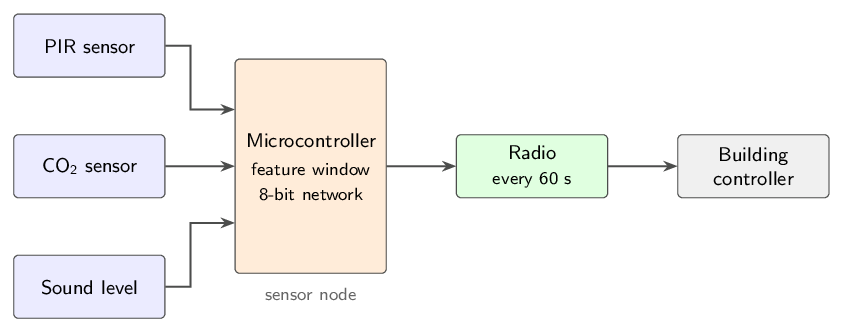
\includegraphics[width=\linewidth]{figures/system-overview.png}
  \caption{The sensor node. Three sensors feed a feature window on the microcontroller; one estimate per minute is sent to the building controller.}
  \label{fig:system}
\end{figure}

\subsection{Network}
The input is a $3 \times 60$ window $\mathbf{x}$ holding one minute of readings from each sensor, normalized per channel. Two depthwise-separable convolution layers with 16 and 24 filters are followed by global average pooling and a fully connected layer with five outputs, one for each occupancy class from empty to four or more people. The model has 4.1~thousand parameters.

\subsection{Training Objective}
Counting errors are not equally costly: confusing two people with three matters less than confusing an empty room with an occupied one. We therefore train with a weighted cross-entropy loss
\begin{equation}\label{eq:loss}
  \mathcal{L}(\theta) = -\frac{1}{N} \sum_{i=1}^{N} w_{y_i} \log p_\theta(y_i \mid \mathbf{x}_i) + \lambda \lVert \theta \rVert_2^2 ,
\end{equation}
where $y_i$ is the true class of window $\mathbf{x}_i$, $w_{y_i}$ is the weight of that class, and $\lambda$ controls weight decay. We set $w_0 = 2$ for the empty class and $w_c = 1$ otherwise, and minimize \eqref{eq:loss} with Adam~\cite{kingma2015adam}.

\subsection{Quantization}
After 40~epochs of floating-point training, weights and activations are constrained to 8-bit integers and the model is trained for ten further epochs so that it adapts to the rounding. Algorithm~\ref{alg:inference} lists the steps the node performs every minute.

\begin{algorithm}[t]
\caption{Occupancy estimate on the node, run once per minute}
\label{alg:inference}
\begin{algorithmic}[1]
\Require buffers $B_{\mathrm{pir}}, B_{\mathrm{co2}}, B_{\mathrm{snd}}$ of 60 samples; quantized network $f_\theta$
\Ensure occupancy class $\hat{y} \in \{0, 1, 2, 3, 4\}$
\State $\mathbf{x} \gets \Call{Normalize}{B_{\mathrm{pir}}, B_{\mathrm{co2}}, B_{\mathrm{snd}}}$
\State $\mathbf{p} \gets f_\theta(\mathbf{x})$ \Comment{38 ms on the microcontroller}
\State $\hat{y} \gets \arg\max_c \, p_c$
\If{$\hat{y} \neq \hat{y}_{\mathrm{prev}}$ \textbf{or} 10 minutes since last transmission}
  \State \Call{Transmit}{$\hat{y}$}
  \State $\hat{y}_{\mathrm{prev}} \gets \hat{y}$
\EndIf
\State sleep until the next minute
\end{algorithmic}
\end{algorithm}

\section{Experiments and Results}\label{sec:experiments}
\subsection{Setup}
We installed one node in each of 14 meeting rooms, with capacities from four to twelve people, for twelve weeks. Ground truth came from a ceiling-mounted counter that was installed for the study and removed afterwards. Data from ten rooms was used for training and validation; the remaining four rooms were held out for testing, so that every reported number is for rooms the model had not seen.

\subsection{Accuracy}
Table~\ref{tab:results} compares our model with two baselines: a PIR detector with a 15-minute timeout, and a gradient-boosted classifier over hand-built features that runs on a server. The quantized network loses 0.9 percentage points of detection accuracy against its floating-point version and remains well ahead of both baselines. Fig.~\ref{fig:accuracy} shows validation accuracy during training.

\begin{table}[t]
  \caption{Results on the Four Held-Out Rooms}
  \label{tab:results}
  \centering
  \begin{tabular}{lccc}
    \toprule
    Method & Detection & Count $\pm 1$ & Power \\
           & (\%)      & (\%)          & (mW) \\
    \midrule
    PIR with timeout       & 83.3 & --   & 0.12 \\
    Boosted trees (server) & 90.6 & 79.4 & 4.80 \\
    Ours, floating point   & 95.1 & 88.9 & 0.74 \\
    Ours, 8-bit            & \textbf{94.2} & \textbf{87.6} & \textbf{0.31} \\
    \bottomrule
  \end{tabular}
\end{table}

\begin{figure}[t]
  \centering
  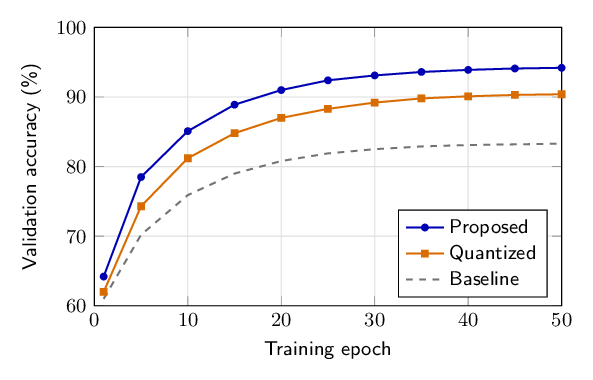
\includegraphics[width=\linewidth]{figures/accuracy.png}
  \caption{Validation accuracy during training. Quantization-aware training recovers most of the accuracy lost to 8-bit rounding.}
  \label{fig:accuracy}
\end{figure}

\subsection{Power and Energy Savings}
The node draws 0.31~mW on average, of which the radio accounts for 41\%. Two AA cells last an estimated 3.4~years. Over the final four weeks we let the estimates control the ventilation rate in seven rooms and kept the schedule in the other seven. Fan energy in the controlled rooms was 23\% lower, and carbon dioxide stayed below 1000~ppm for 99.1\% of occupied time, against 99.4\% under the schedule.

\subsection{Limitations}
All rooms are in one building with one ventilation system, and the study covered spring and early summer only. The count saturates at four or more people, which is enough for ventilation control but not for space-use planning.

\section{Conclusion}\label{sec:conclusion}
A small neural network running on a battery-powered sensor node can tell whether a meeting room is occupied, and roughly by how many people, from three inexpensive sensors. In a twelve-week study the node reached 94.2\% detection accuracy at 0.31~mW and cut ventilation fan energy by 23\% without a measurable loss of air quality. We plan to repeat the study over a full heating season and in open-plan areas, where occupancy changes more gradually.


% Thank people and funders who are not authors. Delete the section if it does not apply.
\section*{Acknowledgment}
The authors thank the facilities team at Northfield Institute of Technology for access to the meeting rooms and the building controller logs. This work was supported in part by the Smart Campus Initiative under grant SCI-2024-117.

\bibliographystyle{IEEEtran}
\bibliography{references}

\end{document}
